%----------------------------------------------------------------------------
\chapter{Kiértékelés szintetikus adatokon}\label{chapter:kiertekelesszintetikus}
%----------------------------------------------------------------------------
% végére szekvenciadiagrammok, összehasonlítva az előző fejezet algoritmusával

Ez a fejezet bemutatja a korábbi fejezetekben ismertetett és implementált algoritmusok eredményét különböző általános adathalmazokon. Az ebből kapott eredményeket ismerteti és összehasonlítja egymással.

\section{Adatforrás}
A gépi tanulási algoritmusok bemenete általában egy adatsor. Egy megtisztított adatsort létrejötte egy hosszabb folyamat eredménye. Először adatfelvételt kell végezni, gyakran ezt digitalizálni is szükséges. Ezután a ki kell szűrni a mérési hibákat amennyire lehetséges. A cél egy olyan adatsor, amely nem tartalmaz hiányt és egyik változó szórása sem kiemelkedően magas.

Annak érdekében, hogy az új algoritmusok teszteléséhez, valamint az eredményeik reprodukálásához ne legyen szükség ezeknek a lépéseknek az elvégzésére, léteznek előfeldolgozott adatokat tartalmazó adatbázisok, melyek szabadon hozzáférhetők. Így a reprodukálás is egyszerűbb, mert ugyanazokon az adatokon lehet így futtatni az algoritmusokat.

Az egyik legismertebb és legtöbbet használt ilyen adatbázis az \emph{UCI Machine Learning Repository} \cite{dua2019university}. 1987-ben hozták létre egy ftp-n elérhető archívumként. Jelenleg 588 adatsort tartanak karban. Ismertsége megmutatkozik abban is, hogy a számítástechnikai publikációkban a 100 legtöbbet hivatkozott forrás között szerepel. Emellett a \emph{scikit-learn} python csomag, mely az adattudósok körében szintén gyakran használt könyvtár, több adatsort tartalmaz ebből a tárházból. Ezek a csomag telepítésével automatikusan letöltődnek, mert elég kis méretűek.

\section{Iris}
Az adattárház egyik első adatsora. A különböző nőszirom nemzetségbe tartozó fajokról tartalmaz információkat. Három faj szerepel benne: a mocsári írisz, a foltos nőszirom és a virginiai nőszirom. A fajok példányai a rekordok, mindegyik tartalmazza a példány csészelevelének és sziromlevelének a szélességét és magasságát. A cél megállapítani a növényfajt a kapott csésze- és sziromlevél méretekből.Minden fajhoz 50 adatpont tartozik, így a teljes adatsor 150 mintából áll. Mivel sok más tanulmánnyal is összevethetők így az adatok, az algoritmusok összehasonlításához ez a Diplomamunka is ezt az adatsort használja.

További előnye a kis változószám, amely miatt az eredmények könnyebben áttekinthetők.

\subsection{Referencia}
A Chen et al. \cite{chen2017learning} és a \ref{chapter:bayesdontesalapu}. fejezet által ismertetett módszer eredményei szerepelnek ebben a szakaszban. A tanulmányban leírt módokon futott, hogy az implementáció sikerességét empirikusan is meg lehessen tapasztalni. Az így kapott eredményeket össze lehet hasonlítani más tanulási módokkal, így a kiértékelésnél ez van először bemutatva.

A bemutatott két módszer egyike az ismert topológiai sorrendű struktúrán tanulás, a másik minden előzetes információ nélkül, a legjobb értékelésűt kiválasztva.

Az ismert topológiai sorrend a \emph{E, A, B, C, D} amennyiben az oszlopokat ábécé szerint nevezzük el. Tehát a faj az első, ennek leszármazottjait keressük. Ezzel a sorrenddel k2 struktúra tanulás fut, mely közben minden él hozzáadása után lefut a diszkretizáló algoritmus. A struktúra tanulás következő lépése már a frissített diszkretizációval rendelkező adatokkal számol.

Az előzetes információk nélküli tanulás esetén 50 véletlenszerű topológiai sorrenddel futott a k2 algoritmus. Minden él hozzáadása után ebben az esetben is diszkretizáció következett, a frissített diszkretizációs elv alapján számolt adatokon. Öt változó esetén az összes lehetséges topológiai sorrend $5! = 120$ lenne, így a futtatáskor csak 42\%-a van tesztelve. Ezért előfordulhat, hogy több futtatás esetén különböző az eredmény. A kapott 50 struktúrához a k2 algoritmus heurisztikája értékeinek összegét rendeli. Ez alapján a legmagasabb értékű lesz a kiválasztott sorrend és struktúra.

\begin{figure}[htp]
    \centering
    \includegraphics[width=12cm]{figures/result/ref_adott.png}
    \caption{Referencia módszer szerint, ismert topológiai sorrend mellett kialakított Bayes-háló}
    \label{fig:eredmeny-referencia-ismert}
\end{figure}

\begin{table}[htp]\centering
    \begin{tabular}{lcc}
    Változó               & Ismert     & Véletlenszerű \\ \hline
    Csészelevél hossz     & 5.45, 6.15 & 5.45, 6.15   \\
    Csészelevél szélesség & 2.95, 3.35 & 2.95, 3.35   \\
    Sziromlevél hossz     & 2.45, 4.75 & 2.45, 4.75   \\
    Sziromlevél szélesség & 0.80, 1.75 & 0.80, 1.75
    \end{tabular}
    \caption{Referencia módszer szerint, ismert és véletlenszerű topológiai sorrend mellett számolt referenciatartományok a folytonos változókra}
    \label{tab:eredmeny-referencia}
\end{table}

Az ismert topológiai sorrend melletti futás nagyon gyors volt. Az inicializáció és a végleges diszkretizáció között 1,937 másodperc telt el.

Az automatikus tanulás során az eltelt időre a korábbi ötvenszerese várható, hiszen azt az algoritmust futtatjuk ötvenszer. A 2 perc 11 másodperces futásidő ennél lényegesen hosszabb (2s * 20 = 100s = 1m 40s). Ennek oka, hogy az ezalatt tanult bayes-hálók bonyolultabbak, mint az ismert sorrendű egy szülős felépítése. Az algoritmus pedig a közös gyerek szüleit lassan diszkretizálja. A véletlenszerű struktúrák esetén pedig ilyenek könnyen előfordulhatnak.

\begin{figure}[htp]
    \centering
    \includegraphics[width=12cm]{figures/result/ref_random.png}
    \caption{Referencia módszer szerint, véletlenszerű topológiai sorrendből a legjobb mellett kialakított Bayes-háló}
    \label{fig:eredmeny-referencia-random}
\end{figure}

A véletlenszerű topológiai sorrendekből az algoritmus szerint a \emph{E, B, D, A, C} bizonyult a legjobbnak. Az ebből kialakított Bayes-háló struktúra a \ref{fig:eredmeny-referencia-random}. ábrán látható. Hasonló az ismert struktúrához, de a sziromlevél szélesség és a csészelevél hossza között összefüggést ismert fel. A kialakult diszkretizáció megegyezik az ismert sorrenddel számolt diszkretizációval, ezért tekinthetjük ezt a referencia diszkretizációnak.
% TODO: összefüggés ábrán

\subsection{Egyváltozós diszkretizáció}
Egy egyszerű módszer a folytonos adatsorból Bayes-háló tanulására az egyváltozós diszkretizáció. A \ref{chapter:jelenlegimodszerek}. fejezet ismertetett két egyszerű módszert ehhez a feladathoz. A nyomaték párosítás komplexitása miatt algoritmikusan nehezen megvalósítható. A tárgyterület-függő diszkretizáció pedig általánosan nem alkalmazható.

Az egyváltozós diszkretizáció után kapott diszkrét adatsor felhasználható a különböző struktúra tanuló algoritmusok bemeneteként. Ilyenkor elég egyetlen alkalommal futtatni a struktúra tanulást, hiszen a diszkretizációs algoritmus eredménye független a struktúrától. Az így kapott Bayes-hálót értékelhetjük.

\begin{table}[htp]\centering
    \begin{tabular}{lccc}
        Változó               & Referencia & Egyenlő hosszú & Egyenlő mintaszámú \\ \hline
        Csészelevél hossz     & 5.45, 6.15 & 5.50, 6.70     & 5.40, 6.30                              \\
        Csészelevél szélesség & 2.95, 3.35 & 2.80, 3.60     & 2.90, 3.20                              \\
        Sziromlevél hossz     & 2.45, 4.75 & 2.97, 4.93     & 3.00, 4.90                              \\
        Sziromlevél szélesség & 0.80, 1.75 & 0.90, 1.70     & 1.00, 1.60                              \\
    \end{tabular}
\caption{Egyváltozós diszkretizációk és a referencia eredménye a diszkretizációs határok}
\label{tab:eredmeny-egyvaltozos}
\end{table}


Az egyenlő széles és az egyenlő mintaszámú diszkretizációk eredményét a \ref{tab:eredmeny-egyvaltozos}. táblázat ismerteti. Az intervallum határok között kisebb eltérések láthatók. Általában a referencia vágópontjai alacsonyabbak, mint az egyváltozós vágások. A futásidő rendkívül rövid, mivel egy diszkretizációs és egy struktúra tanuló lépés fut csak. Minden esetben 0.071 másodperc körüli idő alatt elkészült a Bayes-háló.

\begin{figure}[htp]
    \centering
    \includegraphics[height=12cm]{figures/result/eq_width-greedy.png} \hfill
    \includegraphics[height=12cm]{figures/result/eq_width-chowliu.png}
    \caption{Egyváltozós diszkretizáció Bayes-hálói. Balra az \emph{exact} és a \emph{greedy}, jobbra a \emph{Chow-Liu} algoritmus által tanult háló gráfja.}
    \label{fig:eredmeny-egyvaltozos}
\end{figure}

Négy különböző struktúra tanuló algoritmussal kiértékelve mindkét diszkretizációs elvet a \ref{fig:eredmeny-egyvaltozos}. ábrán látható Bayes hálók készültek az \emph{exact, greedy} és \emph{Chow-Liu} algoritmusokkal. A különbség kizárólag az élek irányában van, egymás transzponáltjai \cite{essam1970some}. A \emph{k2} algoritmus (a \emph{E, A, B, C, D} topológiai sorrenddel) ugyanazt a hálót alkotta, mint a referencia esetben, ami a \ref{fig:eredmeny-referencia-ismert}. ábrán látható. Az algoritmusok eredménye a diszkretizációtól nem változott meg, a különbségek nem voltak ehhez elég erőteljesek.

\subsection{Eredmény}
Az algoritmusok értékelése az implementált értékelő kimenete alapján történt. A vizsgálat tízszeres kereszt-validációt alkalmazott. Ez azt jelenti, hogy a teljes adathalmaz $\frac{9}{10}$ része vesz részt egyszerre a Bayes-háló tanításában. A maradék $\frac{1}{10}$ rész csak a tanítás után van átadva a diszkretizálónak. Ilyenkor a folytonos változókat a tanult diszkretizációs elv alapján rendezi csoportokba. Ezután a diszkretizált értékek alapján a betanított Bayes-háló kiadja a célváltozó (eredetileg diszkrét változó) legvalószínűbb értékét. A kapott és a valós értékeket a meghatározott metrikák \cite{powers2020evaluation} szerint kiértékeli.

\begin{table}[htp]\centering
    \begin{tabular}{lccc}
        Metrika                         & Referencia & Egyenlő hosszú & Egyenlő mintaszámú \\ \hline
        Valódi pozitív                  & 139.00     & \textbf{147.00}         & 139.00             \\
        Hamis pozitív                   & 11.00      & \textbf{3.00}           & 11.00              \\
        Valódi pozitív arány            & 0.93       & \textbf{0.98}           & 0.93               \\
        Hamis felfedezési arány         & 0.07       & \textbf{0.02}           & 0.07               \\
        Pozitív prediktív érték         & 0.93       & \textbf{0.98}           & 0.93               \\
        Pontosság                       & 0.95       & \textbf{0.99}           & 0.95               \\
        Matthews korrelációs együttható & 0.89       & \textbf{0.97}           & 0.89               \\
        F-pontszám                      & 0.93       & \textbf{0.98}           & 0.93
    \end{tabular}
\caption{Kiértékelés eredménye egyváltozós diszkretizációk esetén. \textbf{Félkövérrel} az adott metrika szerinti legjobb eredmény szerepel.}
\label{tab:kiertekeles-egyvaltozos}
\end{table}

A kiértékelés eredménye a \ref{tab:kiertekeles-egyvaltozos}. táblázatban található. A struktúra tanuló algoritmus az elért eredményeken nem változtatott, csak a diszkretizáció módosított rajta. Látható, hogy az egyenlő mintaszám alapján készült diszkretizáció ugyanolyan pontszámot ért el, mint a referencia módszer. Az egyenlő hosszú intervallumokkal dolgozó pedig mindkettőnél sokkal pontosabb volt.

\begin{figure}[htp]\centering
    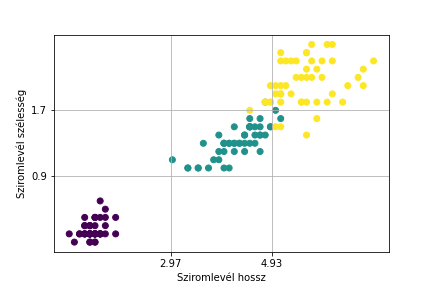
\includegraphics[width=12cm]{figures/IrisEloszlas.png}
    \caption{Iris adathalmaz sziromlevél hossz és sziromlevél szélesség változóinak együttes eloszlása az egyenlő hosszú diszkretizációs elv szerint. A különböző színek a különböző fajokat jelölik.}
    \label{fig:iris-eloszlas}
\end{figure}

Az egyenlő hosszú intervallumokkal dolgozó algoritmus jó eredményének az oka a \ref{fig:iris-eloszlas} ábrán látható. Ez az ábra az adatsor sziromlevél hossz, sziromlevél szélesség és faj változójának értékei alapján jelöli az adatpontokat. A két folytonos változó értéke határozza meg a pozíciót a grafikonon, míg a pont színe jelöli a fajt. A háttér vonalai az egyenlő hosszú diszkretizációs intervallum határokat jelölik.

Látható, hogy a két folytonos változó szerint a fajok elég nagy mértékben elkülönülnek. Az adatsor felépítése miatt, mivel minden fajból azonos mennyiségű példány szerepel, az egyenlő mintaszámú algoritmus ennyire elkülönülő csoportok esetén megtalálja a megfelelő határokat. A sárga és a zöldeskék pontok lineárisan nem szeparábilisek, ezért hibák mindegyik algoritmusnál előfordulnak. Az egyenlő hosszú algoritmusnak pedig "szerencséje" van ezzel az adatsorral, mert egy-egy folytonos változó egyenletes eloszlású és a fajok egy-egy harmadba esnek. Így sikerül jobb eredményt elérnie, mint a másik két eset.

Összefoglalva az látható, hogy egy egyszerű adathalmazon, melyben a minták jól elkülönülnek, a Bayes-döntés alapú diszkretizációs módszer nem tud jobb eredményt elérni, mint egy egyszerűbb algoritmus. Sőt, egyes esetekben jobb megoldást találhat egy egyváltozós diszkretizációs eljárás.